\documentclass[tikz,border=10pt]{standalone}
\usepackage{tikz}
\usetikzlibrary{positioning,shapes.geometric}

\begin{document}
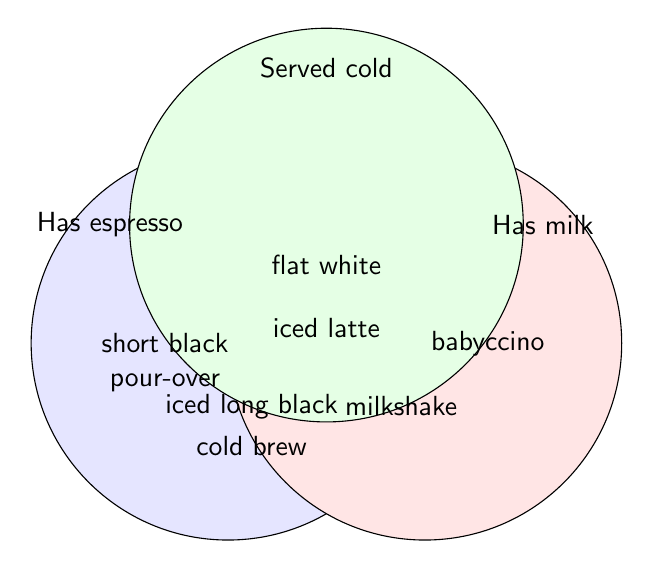
\begin{tikzpicture}[font=\sffamily]

% Draw circles with labels
\draw[fill=blue!10] (0,0) circle (2.5cm);
\draw[fill=red!10] (2.5,0) circle (2.5cm);
\draw[fill=green!10] (1.25,1.5) circle (2.5cm);

% Circle labels (placed outside the circles)
\node at (-1.5,1.5) {Has espresso};
\node at (4.0,1.5) {Has milk};
\node at (1.25,3.5) {Served cold};

% Add drink names in appropriate regions
% Only espresso (left crescent)
\node at (-0.8,0) {short black};
\node at (-0.8,-0.5) {pour-over};

% Espresso + milk (top intersection of left and right circles)
\node at (1.25,1.0) {flat white};

% All three (center)
\node at (1.25,0.2) {iced latte};

% Espresso + cold (bottom-left intersection)
\node at (0.3,-0.8) {iced long black};
\node at (0.3,-1.3) {cold brew};

% Only milk (right crescent)
\node at (3.3,0) {babyccino};

% Milk + cold (bottom-right intersection)
\node at (2.2,-0.8) {milkshake};

\end{tikzpicture}
\end{document}
